\documentclass[conference]{IEEEtran}

\usepackage{enumerate}
\usepackage{enumitem}
\setenumerate[1]{itemsep=0pt,partopsep=0pt,parsep=\parskip,topsep=2pt}
\setitemize[1]{itemsep=0pt,partopsep=0pt,parsep=\parskip,topsep=2pt}
\setdescription{itemsep=0pt,partopsep=0pt,parsep=\parskip,topsep=2pt}

\usepackage{longtable}
\usepackage{rotating}
\usepackage{multirow}
%\usepackage[table]{xcolor}	%for color of table cell
\usepackage{diagbox}		%for head of table

%\usepackage[tight,footnotesize]{subfigure}

\usepackage{listings}
\usepackage{color}

%\usepackage{caption}
\usepackage[noend]{algpseudocode}
\usepackage{algorithm}
\algnewcommand{\LineComment}[1]{\State \(\triangleright\) #1}

\usepackage{amsmath}
\usepackage{amsthm}
\usepackage{multirow}
%\usepackage[amsmath,thmmarks]{ntheorem}

\usepackage{empheq}
\usepackage{xcolor}
\usepackage{graphicx}
\definecolor{hellmagenta}{rgb}{1,0.75,0.9}		%for color of equations
\definecolor{hellcyan}{rgb}{0.75,1,0.9}
\definecolor{hellgelb}{rgb}{1,1,0.8}
\definecolor{colKeys}{rgb}{0,0,1}
\definecolor{colIdentifier}{rgb}{0,0,0}
\definecolor{colComments}{rgb}{1,0,0}
\definecolor{colString}{rgb}{0,0.5,0}
\definecolor{darkyellow}{rgb}{1,0.9,0}

\usepackage{amssymb}
\usepackage{stfloats}
%\usepackage[square, comma, sort&compress, numbers]{natbib}
\usepackage{mathrsfs}
\usepackage{subfigure}

\usepackage{lipsum}
\usepackage{lmodern}
\usepackage{tcolorbox}
\usepackage[linewidth=1pt]{mdframed}

%\usepackage[colorlinks,
%            linkcolor=red,
%            anchorcolor=blue,
%            citecolor=green]{hyperref}

%\usepackage[citecolor=black]{hyperref}
\usepackage{url}
\usepackage{array}
\usepackage{fancyhdr}
\usepackage{booktabs} % For formal tables
\usepackage{textcomp}

\def\BibTeX{{\rm B\kern-.05em{\sc i\kern-.025em b}\kern-.08em
		T\kern-.1667em\lower.7ex\hbox{E}\kern-.125emX}}

\begin{document}

\title{ACETA: Accelerating Encrypted Traffic Analytics on Network Edge}
%\titlenote{Produces the permission block, and copyright information}
%\subtitle{Extended Abstract}

\author{
  \IEEEauthorblockN{Derek Manning\IEEEauthorrefmark{1}, Peilong Li\IEEEauthorrefmark{1}}
  \IEEEauthorblockA{Department of Computer Science\\
    \textit{Elizabethtown College} \\
    \IEEEauthorrefmark{1}\{$ManningD1$, $LiP$\}@etown.edu
  }
  \and
    \IEEEauthorblockN{Xiaoban Wu\IEEEauthorrefmark{2},  Yan Luo\IEEEauthorrefmark{3}}
    \IEEEauthorblockA{Electrical and Computer Engineering\\
  	\textit{University of Massachusetts Lowell} \\
  	\IEEEauthorrefmark{2}$Xiaoban\_Wu$@student.uml.edu, \\
  	\IEEEauthorrefmark{3}$Yan\_Luo$@uml.edu 
  }
  \and
  	\IEEEauthorblockN{Tong Zhang\IEEEauthorrefmark{4},  Weigang Li\IEEEauthorrefmark{4}}
  	\IEEEauthorblockA{
  		\textit{Intel Corporation} \\
  		\IEEEauthorrefmark{4}\{$Tong2.Zhang$, $Weigang.Li$\}@intel.com
  }
}



\maketitle

\begin{abstract}
Applying machine learning techniques to detect malicious encrypted network traffic has become a challenging research topic. Traditional approaches based on studying network patterns fail to operate on encrypted data, especially without compromising the integrity of encryption. In addition, the requirement of rendering network-wide intelligent protection in a timely manner further exacerbates the problem. In this paper, we propose to leverage x86 multicore platforms provisioned at enterprises' network edge with the software accelerators to design an encrypted traffic analytics (ETA) system with accelerated speed. Specifically, we explore a suite of data features and machine learning models with an open dataset. Then we show that by using Intel DAAL and OpenVINO libraries in model training and inference, we are able to boost the training and inference performance time by a maximum order of 32x and 46x respectively. 

\end{abstract}


\begin{IEEEkeywords}
Encrypted Traffic Analysis; DAAL; OpenVINO; Edge Computing; uCPE;
\end{IEEEkeywords}

\section{Introduction and Motivation}
\label{sec:intro}

Encrypted network traffic is the major form of the data transmitting over the Internet today. According to the statistics, 94\% of all Google web traffic is encrypted \cite{google:https} as of July 2019. In 2019 alone, the encryption certificates issued per day is over 1 million \cite{letsencrypt}. While protecting the privacy and providing security for enterprises, encryption technology also benefits evaders to secure their malicious activities. 

Traditional solutions to identify network threats fall into two major categories: 1) deep packet inspection and signatures; and 2) offline network pattern modeling. However, the first category is not applicable on encrypted traffic. Furthermore, solutions that work on decrypted network data will compromise the user privacy and data integrity, and are computationally intensive. By passively monitoring malicious behaviors on a session-based level, the second category of traditional solutions \cite{Anderson:2016, Anderson:2017} demonstrate high accuracy and low false positives. However, training machine learning models, and inferencing with effective models in a timely fashion are challenging due to the high computational power and low response latency requirements.  

With the recent adoption of network function virtualization (NFV) technology, enterprises start to deploy universal customer premises equipment (uCPE) on their network edge to perform complex network functionality including encrypted traffic analytics (ETA) \cite{cisco:eta, intel:ucpe, adva:ucpe}. Such uCPE equipments rely on commodity x86 platforms to enable virtual network functions provisioned without pre-configuration or manual operations. Meanwhile, recent innovation on x86 multicore systems, such as the Intel Data Analytics Acceleration Library (DAAL) \cite{daal} for machine learning and the Intel OpenVINO toolkit \cite{openvino} for computer vision and neural networks, have enabled ETA to render faster training and inference and analyze larger data sets with available compute resources on x86 uCPE equipments. The library also exploits the next-generation processors such as Intel Xeon D \cite{xeond} to render optimal performance. By exploiting DAAL and OpenVINO, we can greatly accelerate the ETA speed without compromising performance.

In this paper, we propose to leverage Intel x86 multicore platforms with the aforementioned software to design an ETA system named \texttt{ACETA} with accelerated model training and inference. Specifically, we contribute in the three following aspects. 1) We seek to study the Cisco’s open-sourced ETA software named \texttt{Joy} \cite{joy} as the reference design, and extend Joy with three new machine learning models and test them with a new open-source dataset. 2) We optimize the ETA pipeline in the proposed software package \texttt{ACETA} with multithreading and Intel software packages to render faster training and inference speed without sacrificing performance. 3) We conduct thorough performance evaluation and comparison between \texttt{Joy} and \texttt{ACETA} for future reference.   

The rest of the paper is organized as follows. Section \S \ref{sec:related} introduces the prior arts. Section \S \ref{sec:design} depicts the overall design of \texttt{ACETA} and its advantages. We evaluate the performance of \texttt{ACETA} in Section \S \ref{sec:eval}. Finally, we conclude the paper in Section \S \ref{sec:concl}.
\section{Related Works}
\label{sec:related}

Anderson et al. \cite{Anderson:2016, Anderson:2017} present a collection of supervised machine learning algorithms for ETA. The authors highlighted two primary reasons why traditional pattern matching approaches cannot be applied to ETA, namely, inaccurate ground truth and a highly non-stationary data distribution. To address the aforementioned problems, the authors develop supervised machine learning models that leverage a unique and diverse set of network flow data features, including 1) TLS handshake meta-features, 2) DNS contextual flows linked to the encrypted flow, 3) HTTP headers of HTTP contextual flows from the same source IP address within a 5-minute window, and 4) META feature. Experiment results show that by incorporating the contextual information into a supervised learning system, the ETA system can achieve 0.00\% false discovery rate and high detection accuracy. 

\texttt{Joy} \cite{joy} is an open-sourced software initiated by the same authors Anderson et al. \cite{Anderson:2016, Anderson:2017}. Though lacking of the network traffic data for reference, the published version of Joy is capable of generating the aforementioned data features. In this paper, we leverage Joy as the feature extraction stage of the \texttt{ACETA} pipeline, and extend the only model published in Joy, namely logistic regression, to a suite of machine learning/deep learning models. More importantly, we implemented an accelerated version of the model suite with Intel DAAL and OpenVINO, and conduct extensive performance study over a public dataset \texttt{CICAndMal2017} \cite{cicandmal2017}.
\section{Design}
\label{sec:design}

In this section, we present the design of \texttt{ACETA} by firstly describing the ETA pipeline and feature generation of Cisco \texttt{Joy}. Then we explain each of the pipeline components of \texttt{ACETA} in detail. 

\subsection{Reference Design - \texttt{Joy}}
As shown in Figure \ref{figure:joy}, the pipeline processing of \texttt{Joy} starts with having the labelled training data collected in packet capture (.pcap) format. Then, using the feature extractor from \texttt{Joy}, the raw data is processed to generate flow level statistics, which is then used to form the features in a structured JSON format. At this point the user can solicit which features to use on the model for training and classification of samples. Once the data features for each of the samples are prepared, a model is trained, tested, and saved for further inference.

\begin{figure}[h!]
  \centering
  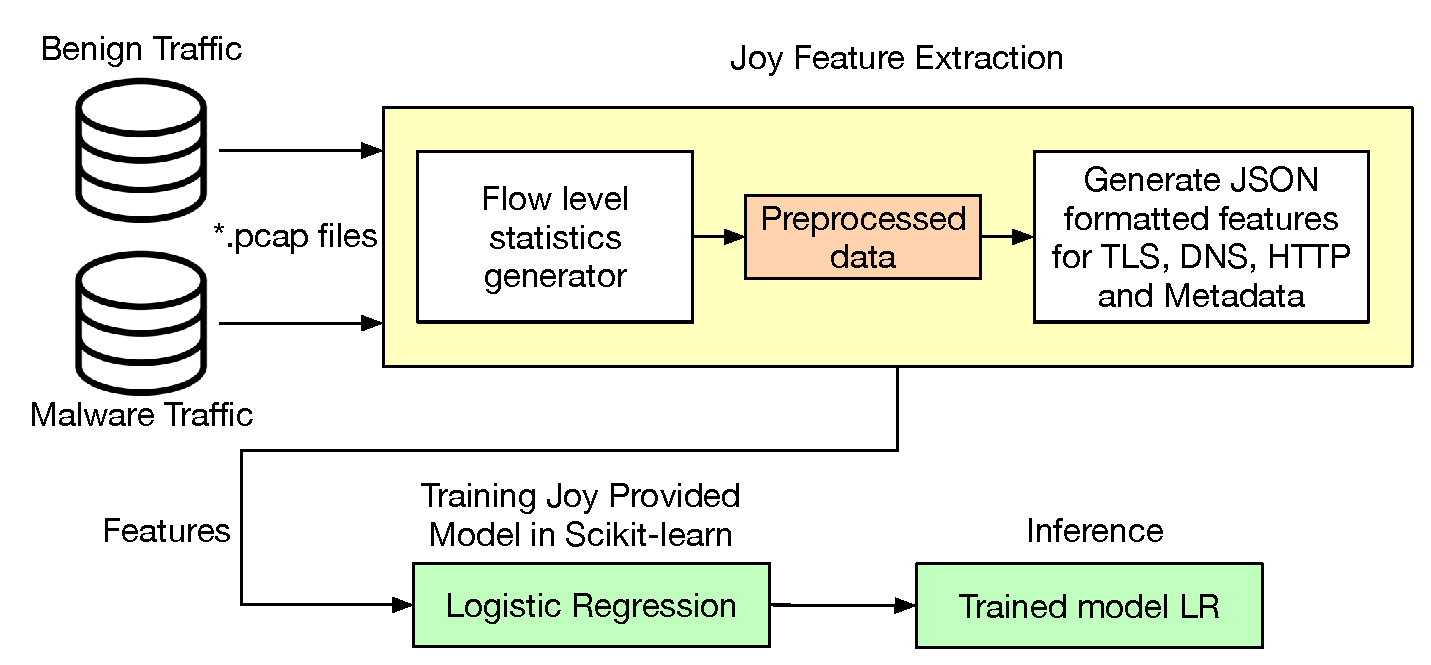
\includegraphics[width=3.3in]{./fig/joy-pipeline.eps}
  \caption{ETA Pipeline of Cisco \texttt{Joy}}
  \label{figure:joy}
\end{figure}

\subsection{Features}

The feature extractor of \texttt{Joy} is capable of extracting TLS, DNS, HTTP and metadata features from network flows. The TLS client-based features are the list of offered ciphersuites, advertised extensions, and the client's public key length, while the server-side TLS features are the selected ciphersuite, supported extensions, number of certificates, number of SAN names, validity in days, and the existence of a self-signed certificate. The DNS flow data is gathered from the corresponding DNS response to the TLS flow. From this flow the gathered features are the lengths of both the domain name and FQDN, the 32 most common TTL values, and binary features representing whether the domain name was in the top-100, top-1,000, top-10,000, top-100,000, top-1,000,000, or not contained in the Alexa list. HTTP data is collected from the source address of every TLS flow. Seven main types of features are used out of the flow data, which are the presence of outbound and inbound HTTP fields, Content-Type, User-Agent, Accept-Language, Server, and code. For metadata, features include the sequence of packet lengths, inter-arrival times, and byte distribution. 

A comprehensive list of features used in \texttt{ACETA} can be found from the list below.

\begin{itemize}
	\item
	The TLS features include:
	1) Client advertised ciphersuites;
	2) Client advertised extensions;
	3) Server supported ciphersuites;
	4) Server supported extensions;
	5) Client public key length;
	6) Number of server certificates;
	7) Number of subject alternative names (SAN) of server;
	8) Validity of server certificates; and
	9) Whether the certificate is self signed.
	\item
	The DNS features include: 
	1) Length;
	2) Suffix;
	3) TTL;
	4) Number of numerical character;
	5) Number of Non-alphanumerical character;
	6) Number of IPs returned per request; and
	7) Alexa rank.
	\item
	The HTTP features include:
	1) Presence of HTTP fields;
	2) Content-type;
	3) User-agent;
	4) Server; and
	5) Return code.
	
	\item
	The metadata features include: 
	1) Inter-Packet Times Markov Matrix;
	2) Inter-Packet Lengths Markov Matrix; and
	3) Byte Distribution.
\end{itemize}

\subsection{\texttt{ACETA} Overview}

As shown in the Figure \ref{figure:aceta}, \texttt{ACETA} improves upon the baseline \texttt{Joy} by accelerating the processing steps at different levels. The initial processing with the \texttt{Joy} tool is accelerated by taking advantage of multicore processors, using multithreading. Likewise, each of the feature processing steps are accelerated by using multiple processes as well. The data processing steps of \texttt{ACETA} use JSON files as the structured storage for our processed data. With the large number of reads and writes our tool needs to complete, the standard JSON library was a substantial bottleneck in the data processing pipeline. Using the C optimized Ultra JSON (ujson) library as a drop in replacement, we gain faster processing with identically structured results. With the data prepared, using the Intel Data Analytics Acceleration Library \cite{daal}, we can accelerate the training and testing of models significantly faster than the standard machine learning libraries.

\begin{figure}[h!]
	\centering
	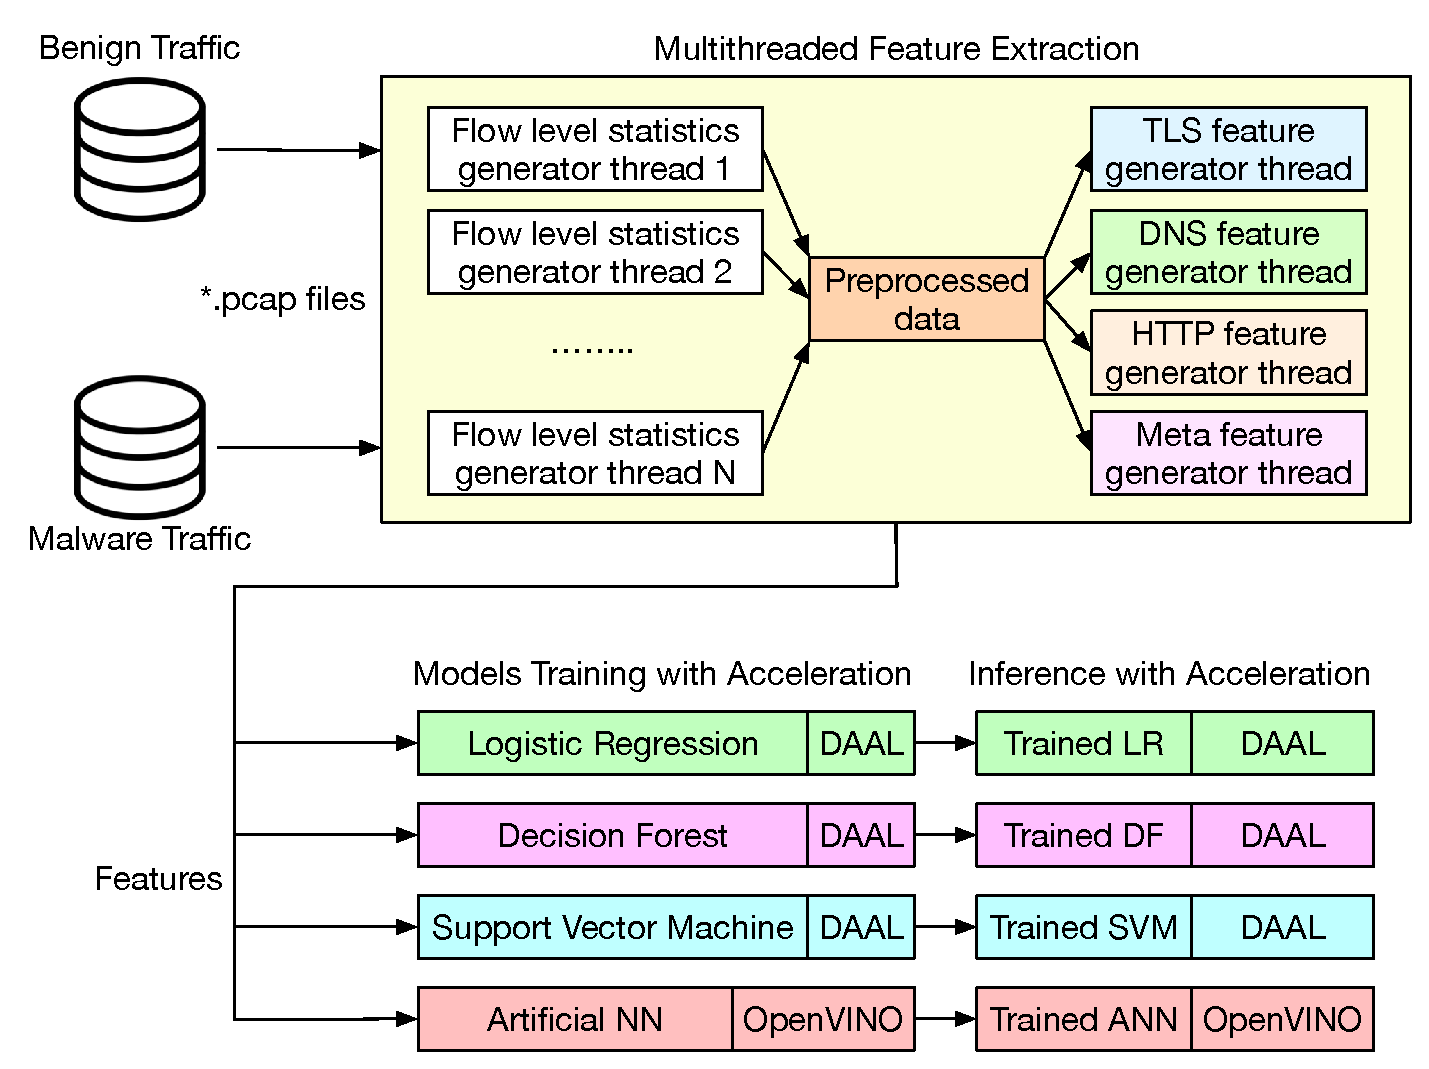
\includegraphics[width=3.3in]{./fig/aceta-pipeline.eps}
	\caption{ETA Pipeline of \texttt{ACETA}}
	\label{figure:aceta}
\end{figure}

\subsection{Acceleration}
Our initial optimizations target the first few data processing steps in \texttt{ACETA}. The performance is enhanced by using several different strategies. First, the code is simplified by implementing faster coding alternatives, such as list comprehensions and conditional exectution using try-catch. Next, the performance libraries Numpy and UltraJSON are implemented for further acceleration. With raw data samples being separated into their unique malware/benign family folders, the organizational structure of the raw data is established effectively to be processed in parallel. Using the multiprocessing library, the parallel capability of multicore machines are leveraged for additional performance gains.

After processing the raw data, the primary focus is on accelerating the model training and inference. The Intel Data Analytics Acceleration Library (DAAL)  \cite{daal} provides optimized machine learning routines and algorithms targeted for Intel processors. DAAL functions maximize processing speed by knowing the instruction set, vector width, core counts, and memory architecture for each processor they run on. Similar to the popular Scikit-learn library, DAAL offers support for many of the popular machine learning algorithms. For our purposes, we compare logistic regression, decision forest, support vector machine, and neural network, by training on identical datasets with both non-DAAL and DAAL version code.

The DAAL machine learning pipeline was designed closely based off of the current popular libraries' structure, such as Scikit-learn. A code comparison of DAAL vs. Scikit-learn is shown in Algorithms \ref{alg:sklearn-lr} and \ref{alg:daal-lr}. Both algorithms implement the same general pipeline of creating a model, training the model, and then predicting using the trained model. This similarity makes implementing DAAL into code that uses one of the standard libraries as simple as possible. 

\begin{algorithm}[h!]
	\caption{Scikit-learn code}
	\scriptsize
	\begin{algorithmic}[1]
		\State import sklearn
		\State logreg = sklearn.linear\_model.LogisticRegression(parameters)
		\State logreg.fit(trainData, trainLabels)
		\State predictions = logreg.predict(testData)
	\end{algorithmic}
	\label{alg:sklearn-lr}
\end{algorithm}

\begin{algorithm}[h!]
	\caption{DAAL code}
	\scriptsize
	\begin{algorithmic}[1]
		\State import daal4py
		\State logreg = daal4py.logistic\_regression\_training(parameters)
		\State trainedModel = logreg.compute(trainData, trainLabels)
		\State predictAlg = daal4py.logistic\_regression\_prediction(parameters)
		\State predictResult = predictAlg.compute(testData, trainedModel.model)
		\State predictions = predictResult.prediction
	\end{algorithmic}
	\label{alg:daal-lr}
\end{algorithm}

For deep learning, Intel also offers a dedicated framework, OpenVINO  \cite{openvino}, that optimizes deep learning models in a similar manner to DAAL. OpenVINO has two components, its Model Optimizer and Inference Engine. The optimization process first requires a pre-trained model from one of its supported deep learning frameworks, in our case TensorFlow. First, the TensorFlow must be frozen into a format the Model Optimizer can analyze. The Model Optimizer converts the TensorFlow model to make an optimized intermediate representation based on the trained network topology, weights, and bias values. The newly optimized model is then used by the Inference Engine to classify new data, at a faster rate and with identical accuracy compared to the original TensorFlow model.


\section{Evaluation}
\label{sec:eval}
In this section we evaluate the performance of the proposed ETA system \texttt{ACETA}. In particular we focus on the training time, inference time, accuracy, and performance breakdown of the different steps. First, we cover the experiment background and methodology for executing the comparisons. Then we discuss general performance improvements made in \texttt{ACETA} relative to the \texttt{Joy} baseline. After addressing general improvements, we cover each of the aforementioned performance metrics in detail for each of the models tested.  

\subsection{Experiment Platform and Methodology}
We perform all testing for \texttt{ACETA} on a commodity workstation with Intel x86 processors to resemble the real-world uCPE setting. The Intel Distribution for Python is used in an Anaconda environment for all programming, with all applicable additional packages coming via the Intel channel. The detailed hardware and software specifications are listed in Table \ref{tbl:platform}. We use the \texttt{CICAndMal2017} dataset \cite{cicandmal2017}, provided by the University of New Brunswick, for training and testing in all comparisons . In addition to benign flows, this dataset contains four categories of malware: adware, ransomware, scareware, and SMS malware, with samples coming from 42 unique malware families. Comparing the baseline with \texttt{ACETA} first involves randomly splitting subsets of the processed data for training and testing, providing one sample from each of the malware families per subset, along with many more benign samples. The subsets are partitioned, and then saved to separate files to be shared by the baseline and \texttt{ACETA} for level comparison results. We use the standard Python time library for the timing of model training, and we measure the accuracy by using the labels of 0 and 1 for benign and malicious samples respectively. Performance statistics are gathered using the generic cProfiling Python utility, along with the kcachegrind tool \cite{kcachegrind} to process and present the data. 

\begin{table}[h!]
\scriptsize
\centering
\caption{Experiment Platform Specification}
\begin{tabular}{|c|c|}
  \hline
  Item  & Specification \\
  \hline\hline
  CPU &  Intel Core i5-8600k 6 cores @ 3.60GHz\\
  \hline
  Memory & 16 GB DDR4 @ 2667MHz\\
  \hline
  HDD & 1TB @ 7200RPM\\
  \hline
  Software & Intel DAAL v0.2019.3\\
  \hline
  & Intel OpenVINO v2019.1.144\\
  \hline
  & Anaconda v5.3.0 \\
  \hline
  Host OS & Ubuntu 16.04 Desktop\\
  \hline
\end{tabular}
\label{tbl:platform}
\end{table}

\subsection{Performance Results}
The baseline raw to processed data pipeline takes on average 33.7 minutes for completion. Given this result, we begin to implement strategies to accelerate the pipeline. Initial data processing optimizations such as list comprehensions, string formatting, accelerated conditional processing using try-catch, and using Numpy arrays instead of Python lists improve the average performance to 30.1 minutes, a speedup of 8.3\%. Multiprocessing the initial data processing with \texttt{Joy}, and also the feature analysis result in an average performance of 23.2 minutes, a speedup of 31.2\% relative to the baseline. Next, we exploit the ujson library as a drop-in replacement for the standard JSON library, resulting the process to take only 17.8 minutes, a cumulative speedup of 47.2\%.

\subsubsection{Training Time}
In the model creation phase of \texttt{ACETA}, the user has the option to select which type of model to train and save. Currently, the model options are logistic regression, decision forest, support vector machine, and an artificial neural network. The baseline version of the code uses Scikit-learn library for the models, while \texttt{ACETA} uses DAAL, with both versions' models using identical parameter settings. The log scale training time of each of the models for the two versions are shown in figure \ref{figure:training-time}. For all of the models except the neural network, the \texttt{ACETA} versions outperform the original by several factors: 10x faster for logistic regression, 3.25x faster for decision forest, and 31x faster for SVM. A 100-epoch neural network comparison results in the \texttt{ACETA} version being around twice as slow as the original. One possible reason for this inconsistency is that the original model uses a deprecated, Scikit-learn neural network API, whereas \texttt{ACETA} uses an Intel Python distribution Keras \cite{keras} model. DAAL offers low level APIs, similar to standard TensorFlow, to design neural networks piece-by-piece, but for the sake of simplicity Keras is used in our implementation. However, it is also worth noting that optimizing this TensorFlow based model, using Intel's OpenVINO deep learning framework \cite{openvino}, results in a faster inference time relative to the baseline neural network.

\begin{figure}[h!]
	\centering
	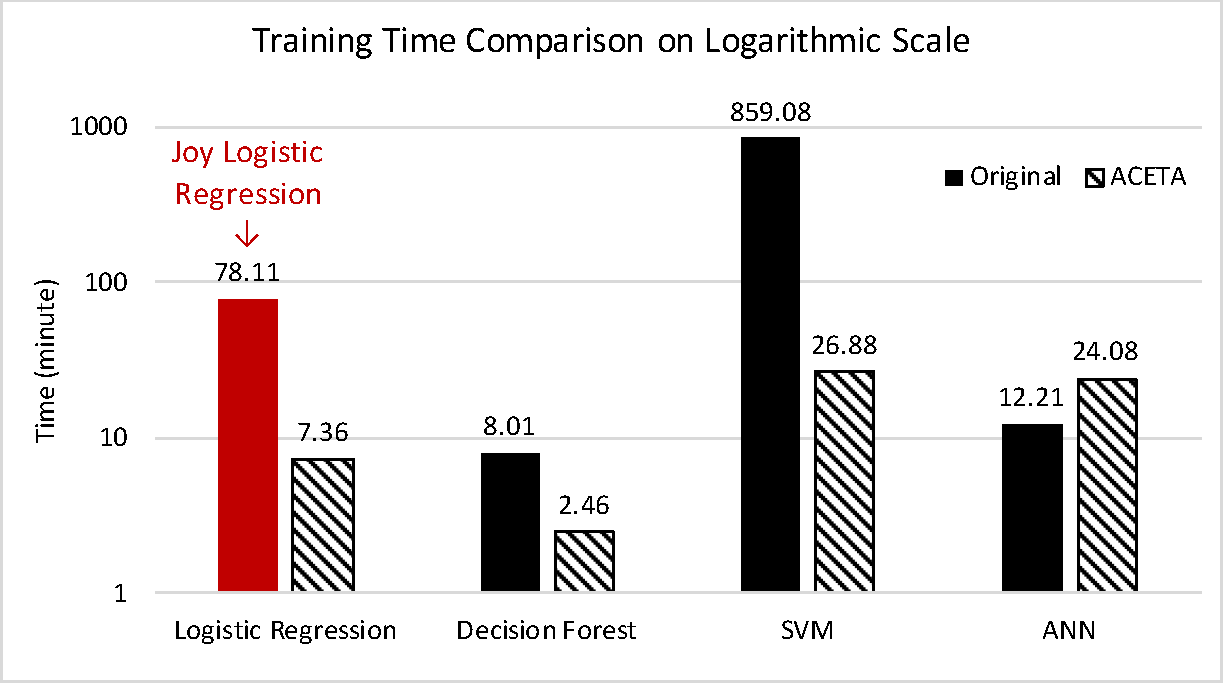
\includegraphics[width=3.3in]{./fig/training-log.pdf}
	\caption{Training Time Comparison on Logarithmic Scale}
	\label{figure:training-time}
\end{figure}

\subsubsection{Inference Time}
In addition to improving training performance, \texttt{ACETA} also performs significantly faster for inference. Figure \ref{figure:inference-time} presents the time comparisons for each model on an identical dataset. The baseline models all complete in roughly 925 milliseconds, compared to the majority of \texttt{ACETA} models taking only 20 milliseconds, a 46x improvement. The only model to underperform is the \texttt{ACETA} ANN, taking about 1.49 seconds to complete its inference (not shown in Figure \ref{figure:inference-time}). However, by optimizing the \texttt{ACETA} Keras/TensorFlow ANN model with Intel OpenVINO, the optimized model inference takes only 30 milliseconds, on the order of the other \texttt{ACETA} models, while retaining the same accuracy as its unoptimized counterpart. 

\begin{figure}[h!]
	\centering
	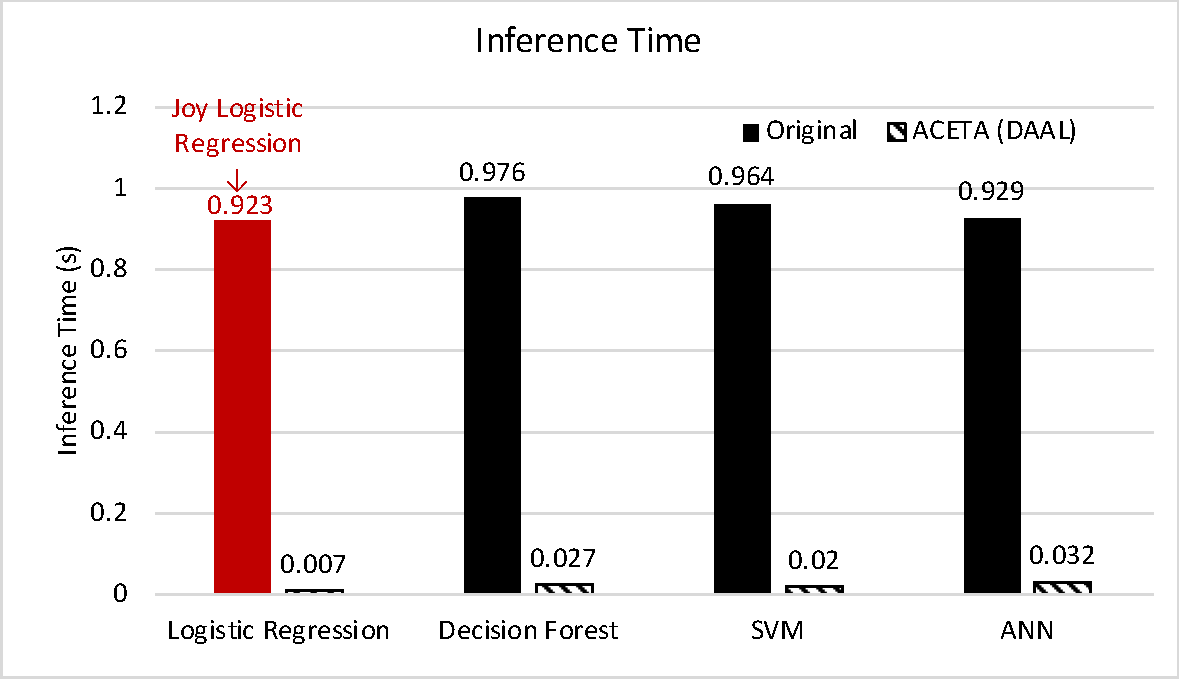
\includegraphics[width=3.3in]{./fig/inference-time.pdf}
	\caption{Inference Time Comparison}
	\label{figure:inference-time}
\end{figure}

\subsubsection{Accuracy}
Figure \ref{figure:training-accuracy} shows accuracy comparisons for model training while Figure  \ref{figure:inference-accuracy} demonstrates inference accuracy on an identical test dataset immediately after model training. With each of the models, the performance shows very little difference between the baseline and \texttt{ACETA}. At most, \texttt{ACETA}'s accuracy is ~2.5\% lower for logistic regression training, but on average the difference is around a single percent. In the case of the decision forest classifier, the \texttt{ACETA} version even outperforms the slower, baseline model. This data, in addition to the training and inference time results, provides significant support for the use of DAAL as an alternative to the standard machine learning libraries.

\begin{figure}[h!]
	\centering
	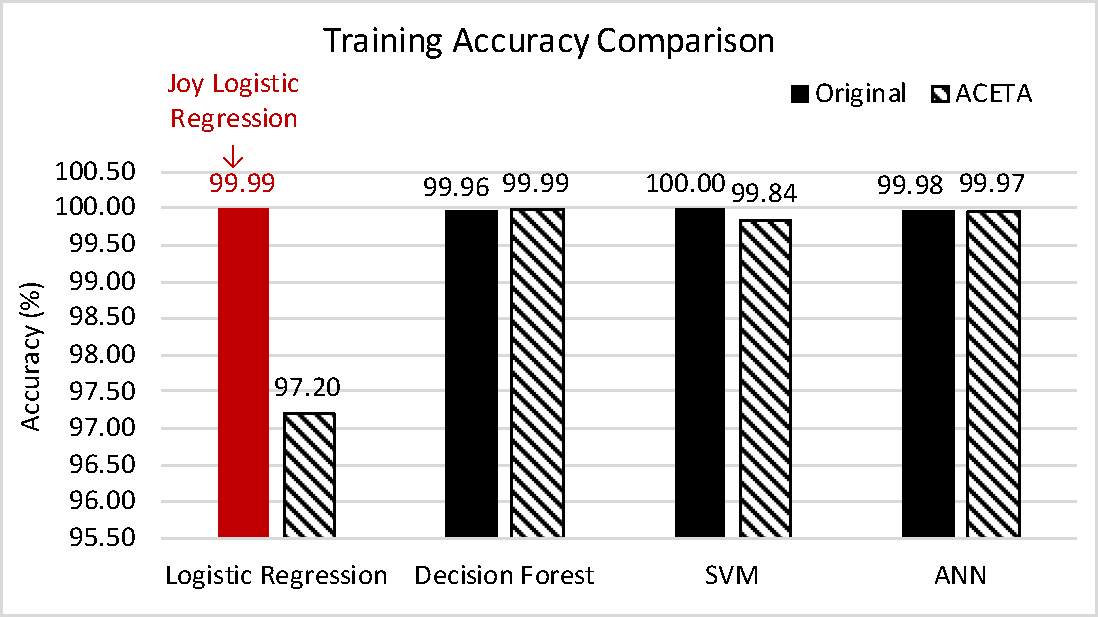
\includegraphics[width=3.3in]{./fig/training-accuracy.pdf}
	\caption{Training Accuracy Comparison}
	\label{figure:training-accuracy}
\end{figure}

\begin{figure}[h!]
	\centering
	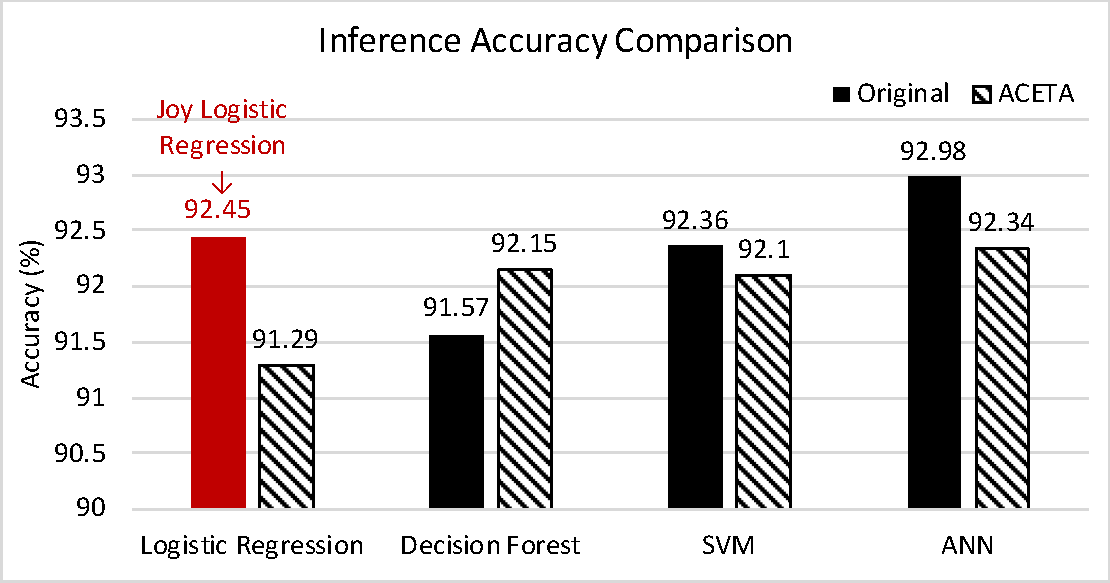
\includegraphics[width=3.3in]{./fig/inference-accuracy.pdf}
	\caption{Inference Accuracy Comparison}
	\label{figure:inference-accuracy}
\end{figure}

\subsubsection{Performance Breakdown}
We leverage the cProfiling utility to track and save the cumulative time the program spends in each of its functions. Using kcachegrind \cite{kcachegrind}, we visualize the data to locate the major hotspots within the training of each of the models. Figure \ref{figure:breakdown} displays this breakdown separated into three categories: training, data preparation, and other. For the majority of the models, the training of the models occupies the biggest percentage of time, which is to be expected. With the acceleration of DAAL and OpenVINO, the \texttt{ACETA} versions receive a great decrease on the overall training time percentage. One interesting observation is the training time percentage of the \texttt{ACETA} decision forest: it is not the most time consuming part of the algorithm. This can be explained by this model being by far the fastest to complete training, so the data processing and overhead inevitably occupy larger percentages of time. With both logistic regression and SVM showing a similar breakdown, the other interesting comparison is between the original and \texttt{ACETA} ANN. As mentioned earlier, the \texttt{ACETA} ANN version uses Keras \cite{keras}, which provides a high-level API to create TensorFlow models. This supports the measured \texttt{ACETA} ANN breakdown that shows a larger percentage of time, 32.3\%, being consumed by other tasks, other being the lump sum of any additional overhead. This irregularity explains at least in part the performance disparity between the baseline and \texttt{ACETA} ANN versions.

\begin{figure}[h!]
	\centering
	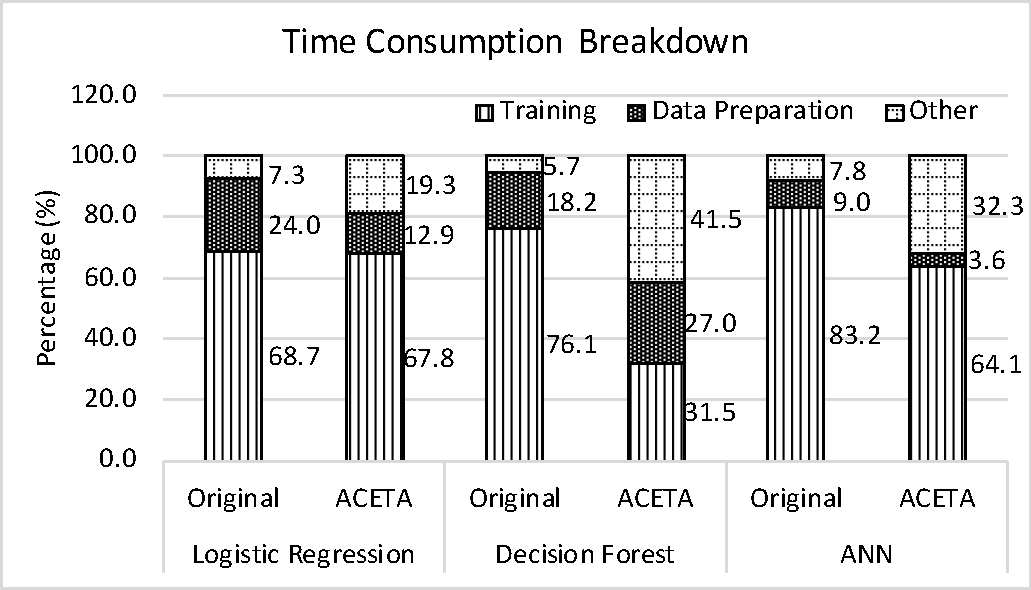
\includegraphics[width=3.3in]{./fig/perf-breakdown.pdf}
	\caption{Time Consumption Breakdown}
	\label{figure:breakdown}
\end{figure}

\section{Conclusion}
\label{sec:concl}

In this paper, we aim to address the challenges in designing a high performance ETA system with the x86 processors provisioned at enterprises' network edge. In the proposed \texttt{ACETA} system, we study machine learning techniques for the identification of encrypted malware network flows. Specifically, we first explore and design multiple sets of features and four machine learning models over a public dataset. We then implement accelerated versions of the four machine learning models without sacrificing classification accuracy using Intel DAAL and OpenVINO. Our experimental results have demonstrated both the feasibility as well as the boosted training and inference performance of such a framework. Going beyond the experiments, our future work will focus on implementing an real-time ETA system for uCPE devices at network edge that comprises of online feature extraction, speeded model training and real-time inference. 

\section*{Acknowledgment}
This work is supported in part by the National Science Foundation (No. 1547428, No. 1541434, No. 1738965 and No. 1450996), a grant from Intel Corporation, and a grant from Summer Scholarship, Creative Arts and Research Projects (SCARP) Program of Elizabethtown College. 


\bibliographystyle{IEEEtran.bst}
\bibliography{ref} 

%\appendix
%
%\subsection{Use Case Demonstration}
%\label{UseCaseAppendix}

%\begin{table}[ht]
%\centering
%\caption{Examples of use cases (based on the topology of Fig. \ref{fig:ex_event} ).}
%\label{table:ex_query}
%\begin{tabular}{|l|p{3.4 in}|l|l|}
%\hline
%\textbf{Example} & \textbf{Query code} & \textbf{Composition} & \textbf{Description} \\ \hline
%\begin{tabular}[c]{@{}l@{}}Flow volume \\ over a link\end{tabular} & \begin{tabular}[c]{@{}l@{}}q1: Select ipv4\_src, ipv4\_dst, AVG(pkt\_len) \\\hspace*{3mm} Where sw\_id=sw1 \& in\_pt=1 \\ Groupby ipv4\_src, ipv4\_dst\end{tabular} & N & \begin{tabular}[c]{@{}l@{}}Query per-flow average \\ volume over a specified link.\end{tabular} \\ \hline
%\begin{tabular}[c]{@{}l@{}}Heavy hitter \\ detection\end{tabular} & \begin{tabular}[c]{@{}l@{}}q2: Select src\_ip, dst\_ip Where hh\_counter \textgreater1G \\ \hspace*{3mm} Groupby src\_ip, dst\_ip\\ create aggregate hh\_counter (agg\_hh):\\ \hspace*{3mm} agg\_hh{[}src\_ip{]}{[}dst\_ip{]} += pkt.pkt\_len\end{tabular} & N & \begin{tabular}[c]{@{}l@{}}Source-destination IP address\\  pairs whose traffic volume is\\  more than a pre-specified\\  threshold.\end{tabular} \\ \hline
%\begin{tabular}[c]{@{}l@{}}Flow volume \&\\  link throughput, \\ sequentially\end{tabular} & \begin{tabular}[c]{@{}l@{}}q3: Select src\_ip, dst\_ip, SUM(pkt\_len) \\ \hspace*{3mm} Where src\_ip=10.0.0.1, dst\_ip=10.0.0.10 \\ Groupby ipv4\_src, ipv4\_dst\\ q4: Select SUM(pkt\_len) Where sw\_id=sw1 \& in\_pt=1 \\ \hspace*{3mm} When q3:true\end{tabular} & q3 $\gg$ q4 & \begin{tabular}[c]{@{}l@{}}Execute two queries\\ sequentially.\end{tabular} \\ \hline
%\begin{tabular}[c]{@{}l@{}}Packet loss \\ detection\end{tabular} & \begin{tabular}[c]{@{}l@{}}q5: Select src\_ip, dst\_ip, pkt\_loss Groupby src\_ip, dst\_ip\\ q6: Select src\_ip, dst\_ip, window\_size Groupby src\_ip, dst\_ip \\ When q5:pkt\_loss\textgreater1000\\ q7: Select src\_ip, dst\_ip, SUM(pkt\_len) Groupby src\_ip, dst\_ip \\ When q5:pkt\_loss\textgreater1000\\ create aggregate pkt\_loss (agg\_pl, agg\_seq) \\ \hspace*{3mm} if pkt.seq $<$ agg\_seq then\\ \hspace*{3mm} agg\_pl++ else \\ \hspace*{3mm} agg\_seq = pkt.seq + pkt.payload\_len \end{tabular} & \begin{tabular}[c]{@{}l@{}}q5 $\gg$ \\ (q6\&q7)|e\end{tabular} & \begin{tabular}[c]{@{}l@{}}When the packet loss of TCP\\  flows exceed a threshold, TCP\\ window size and volume\\  of the flow will be measured.\end{tabular} \\ \hline
%\begin{tabular}[c]{@{}l@{}}Loss localization \\ along a path\end{tabular} & \begin{tabular}[c]{@{}l@{}}q8: Select src\_ip, dst\_ip, pkt\_loss Where ipv4\_src=10.0.0.1 \\ \hspace*{3mm}\& ipv4\_dst=10.0.0.10 \\ Groupby src\_ip, dst\_ip\\ q9: Select src\_ip, dst\_ip, SUM(pkt\_len) Where sw\_id=sw1 \\ \hspace*{3mm} \& in\_pt=1 \\ Groupby src\_ip, dst\_ip When q8: pkt\_loss\textgreater1000\\ q10: Select src\_ip, dst\_ip, SUM(pkt\_len) Where sw\_id=sw2 \\ \hspace*{3mm}\& in\_pt=1 \\ Groupby src\_ip, dst\_ip When q8: pkt\_loss\textgreater1000\end{tabular} & \begin{tabular}[c]{@{}l@{}}q8 $\gg$ \\ (q9\&q10)|e\end{tabular} & \begin{tabular}[c]{@{}l@{}}Measure throughput in \\ different locations along \\ a path when the packet \\ loss of a TCP flow exceeds \\ a threshold.\end{tabular} \\ \hline
%DDoS detection & \begin{tabular}[c]{@{}l@{}}q11: Select dst\_ip, COUNT(SYN) Groupby dst\_ip\\ q12: Select dst\_ip, diff\_syn\_ack Groupby dst\_ip \\ \hspace*{3mm} When q11:COUNT(SYN)\textgreater 1000\\ create aggregate diff\_syn\_ack (agg\_diff,agg\_syn,agg\_ack):\\ \hspace*{3mm}if pkt.SYN=1 \& pkt.ACK=0 then agg\_syn++\\ \hspace*{3mm}if pkt.SYN=1 \& pkt.ACK=1 then agg\_ack++\\ \hspace*{3mm}agg\_diff = agg\_syn - agg\_ack\end{tabular} & \begin{tabular}[c]{@{}l@{}} q11 $\gg$ \\ q12|e \end{tabular} & \begin{tabular}[c]{@{}l@{}}Measure the asymmetry\\  between incoming TCP packets \\ with SYN flags and outgoing\\  TCP packets with SYN and\\  ACK flags.\end{tabular} \\ \hline
%\end{tabular}
%\end{table}

\end{document}
